\documentclass[10pt,landscape]{article}
\usepackage{multicol}
\usepackage{calc}
\usepackage{ifthen}
\usepackage[landscape]{geometry}
\usepackage{amsmath,amsthm,amsfonts,amssymb}
\usepackage{color,graphicx,overpic}
\usepackage{hyperref}
\usepackage{mhchem}
\usepackage{gensymb}
\usepackage{graphicx}

\pdfinfo{
  /Title (example.pdf)
  /Creator (TeX)
  /Producer (pdfTeX 1.40.0)
  /Author (Seamus)
  /Subject (Example)
  /Keywords (pdflatex, latex,pdftex,tex)}

% This sets page margins to .5 inch if using letter paper, and to 1cm
% if using A4 paper. (This probably isn't strictly necessary.)
% If using another size paper, use default 1cm margins.
\ifthenelse{\lengthtest { \paperwidth = 11in}}
    { \geometry{top=.5in,left=.5in,right=.5in,bottom=.5in} }
    {\ifthenelse{ \lengthtest{ \paperwidth = 297mm}}
        {\geometry{top=1cm,left=1cm,right=1cm,bottom=1cm} }
        {\geometry{top=1cm,left=1cm,right=1cm,bottom=1cm} }
    }

% Turn off header and footer
\pagestyle{empty}

% Redefine section commands to use less space
\makeatletter
\renewcommand{\section}{\@startsection{section}{1}{0mm}%
                                {-1ex plus -.5ex minus -.2ex}%
                                {0.5ex plus .2ex}%x
                                {\normalfont\large\bfseries}}
\renewcommand{\subsection}{\@startsection{subsection}{2}{0mm}%
                                {-1explus -.5ex minus -.2ex}%
                                {0.5ex plus .2ex}%
                                {\normalfont\normalsize\bfseries}}
\renewcommand{\subsubsection}{\@startsection{subsubsection}{3}{0mm}%
                                {-1ex plus -.5ex minus -.2ex}%
                                {1ex plus .2ex}%
                                {\normalfont\small\bfseries}}
\makeatother

% Define BibTeX command
\def\BibTeX{{\rm B\kern-.05em{\sc i\kern-.025em b}\kern-.08em
    T\kern-.1667em\lower.7ex\hbox{E}\kern-.125emX}}

% Don't print section numbers
\setcounter{secnumdepth}{0}


\setlength{\parindent}{0pt}
\setlength{\parskip}{0pt plus 0.5ex}

%My Environments
\newtheorem{example}[section]{Example}
% -----------------------------------------------------------------------

\begin{document}
\raggedright
\footnotesize
\begin{multicols}{3}


% multicol parameters
% These lengths are set only within the two main columns
%\setlength{\columnseprule}{0.25pt}
\setlength{\premulticols}{1pt}
\setlength{\postmulticols}{1pt}
\setlength{\multicolsep}{1pt}
\setlength{\columnsep}{2pt}

\begin{center}
     \Large{\underline{Formula Sheet}} \\
\end{center}

\section{returns}

\vspace{0.25cm}

The ``return", $R$, over a single period of any length of time is:

\vspace{0.25cm}

$$R=\frac{V_f - V_i}{V_i}$$

\vspace{0.25cm}

where:

\vspace{0.25cm}

$V_f$ = final value, including dividends and interest

$V_i$ = initial value

\vspace{0.25cm}

The \textbf{log-return}, $R$, is

$$R  = \ln\left(\frac{V_f}{V_i}\right)$$

\vspace{0.25cm}

notice absolute and log returns are not the same thing but they are both denoted by $R$. Basically, its a question of how to \textit{state} your return mathematically.

Logarithmic returns are useful for mathematical finance. One of the advantages is that the logarithmic returns are symmetric, while ordinary returns are not: positive and negative percent ordinary returns of equal magnitude do not cancel each other out and result in a net change, but logarithmic returns of equal magnitude but opposite signs will cancel each other out. \textit{This means that an investment of \$100 that yields an arithmetic return of 50\% followed by an arithmetic return of -50\% will result in \$75, while an investment of \$100 that yields a logarithmic return of 50\% followed by a logarithmic return of -50\% will come back to \$100}

\vspace{0.25cm}

Example absolute R: start with 100. Consider 25\% return (R=0.25). now you have 125. If you follow with a -25\% return (R=-0.25) at this point then you now have 93.75. 

\vspace{0.25cm}

log return: start with 100. Now do a log return of $R=0.25$. So $\ln\left(\frac{V_f}{100}\right) =0.25$ so $V_f = 100e^{0.25} = 128.4$. Now let's follow up with a $R = -0.25$. So $\ln\left(\frac{V_f}{128.4}\right) = - 0.25$ so  $V_f = 128.4e^{-0.25}= 100$. \textit{Voila, mon cherie!}



\section{rates of return}

\vspace{0.25cm}

Without any reinvestment, a return $R$ over a period of time $t$ 
is equivalent to a rate of return:

\vspace{0.25cm}

$\frac{R}{t}$

\vspace{0.25cm}

If there is reinvestment at each step then the rate of return $r$ (not sure how this notation is handled later in the $\beta$ discussion I think they are talking about capital $R$ !? not sure, check that)

\vspace{0.25cm}

$$1+R = (1+r)^t \qquad r = (1+R)^{\frac{1}{t}}-1$$

\vspace{0.25cm}

In these equations, the reinvestment occurs at each step in the unit of time, could be days, months, years. etc. $r$ has units of inverse unit time which will depend on the units.

\vspace{0.25cm}

\textbf{Annualisation} is the process described above, of converting a return 
$R$ to an annual rate of return $r$, where the length of the period $t$ is measured in years and the rate of return $r$ is per year

\vspace{0.25cm}

Suppose a principal amount of \$1,500 is deposited in a bank paying an annual interest rate of 4.3\%, compounded quarterly.
Then the balance after 6 years is found by using the formula above, with P = 1500, r = 0.043 (4.3\%), n = 4, and t = 6: 

$$ P'=1\,500\times \left(1+{\frac {0.043}{4}}\right)^{4\times 6}\approx 1,938.84$$ 

So the new principal, P', after 6 years is approximately \$1,938.84. 
Subtracting the original principal from this amount gives the amount of interest received: 
$1,938.84-1,500=438.84$

\vspace{0.25cm}


Suppose the same amount of \$1,500 is compounded biennially (every 2 years).
Then the balance after 6 years is found by using the formula above, with P = 1500, r = 0.043 (4.3\%), n = 1/2 (the interest is compounded every two years), and t = 6 : 
$$P'=1,500\times \left(1+(0.043\times 2)\right)^{\frac {6}{2}}\approx 1,921.2$$ 

So, the balance after 6 years is approximately \$1,921.24. 
The amount of interest received can be calculated by subtracting the principal from this amount. 
$1,921.24-1,500=421.24$

The interest is less compared with the previous case, as a result of the lower compounding frequency.

\vspace{0.25cm} 

continuously compounded interest rate is called a \textbf{force of interest ($\delta$)} Think about this, what if you took an interest rate, $r$, and broke up some time period. $t$ into infitesimal small units of time e.g. what do you get if you do

$$ \lim\limits_{n\to\infty} (1+\frac{r}{n})^{n t}  = e^{rt}$$

\vspace{0.25cm}  

So the maximum you can get from compounding is this. let's say we took $1500$ and continuously compounded it at the annual rate of 4.3\%, for six years. Then you should get.

$$ 1500 e^{0.043\times6} = 1941.5$$

Notice there is not a big difference in this case between quarterly and continous compounding for this case which is interesting.


\section{Options}

It's important to understand that the value of the option contract will move with the stock price. You can close your position by exercise and assignment. But more likely you can close your position buy \textit{selling the option contract itself before the expiration date without exercise assignment!}. Thus its quite possible that money will change hands without any stocks ever being delivered (assigned)

\vspace{0.25cm}

A \textbf{Call} is a contract between the buyer and seller giving the former the right but not the obligation to buy the underlying stock at a price indicated in the contract despite how high it may be at a time before the contract expires

\vspace{0.15cm}

The seller (writer) of a call has the obligation to fulfill that contract. In a \textit{covered call}, the seller owns the underlying asset and can deliver it if neccessary.

\begin{align*}
\centering
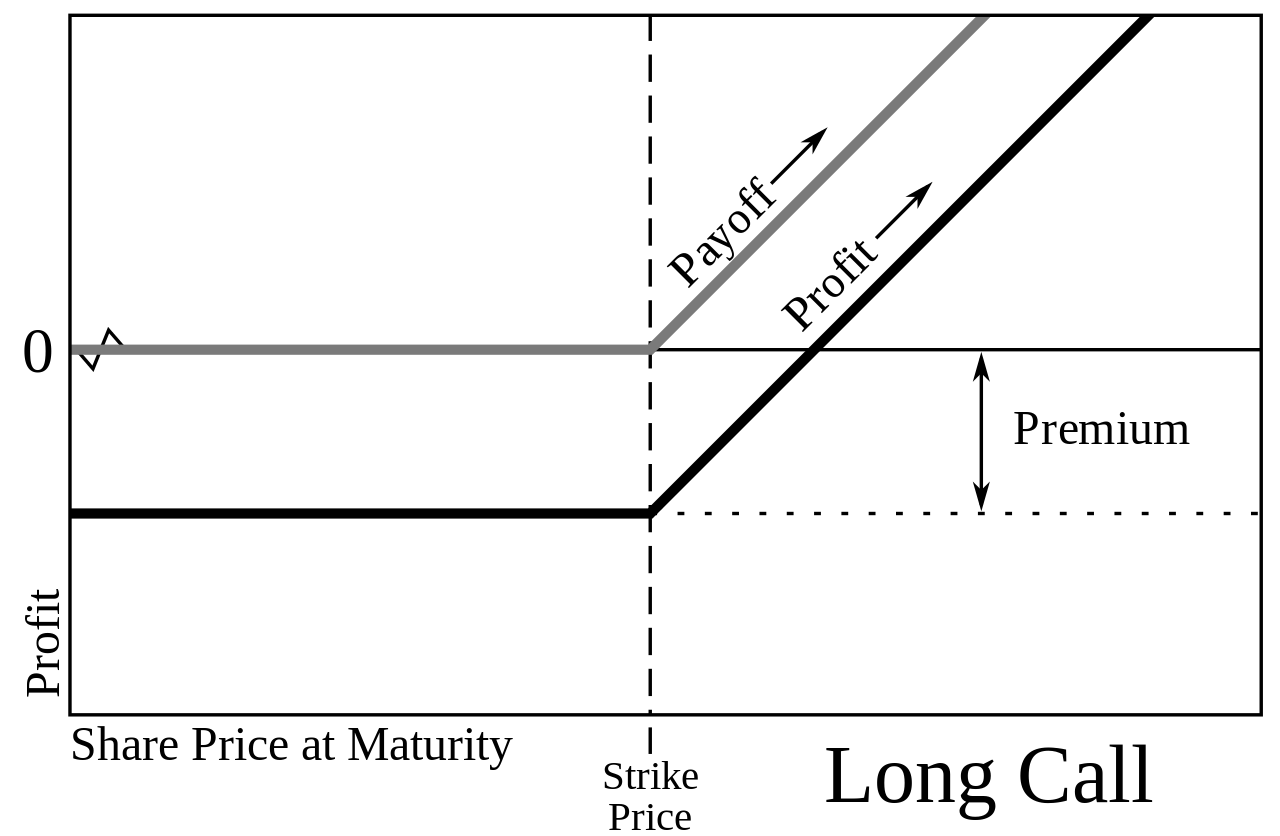
\includegraphics[scale=0.12]{1280px-Long_call_option}
\end{align*}

\vspace{0.15cm}

The profit from buying (going "long" or "Long Call") a call option is shown in the figure above

\vspace{0.15cm}

\begin{align*}
\centering
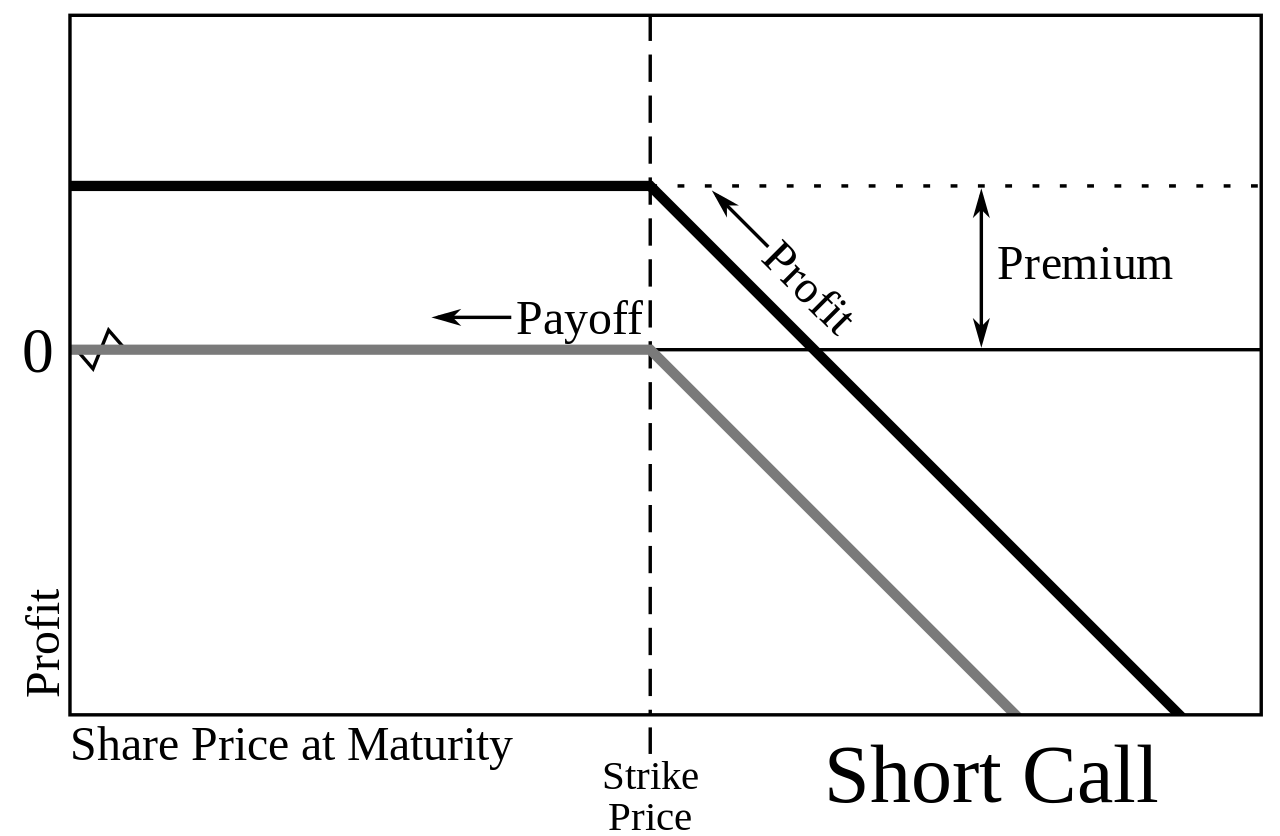
\includegraphics[scale=0.12]{Short_call_option}
\end{align*}

\vspace{0.15cm}

The profit from selling (writing or shorting) a call option is shown in the figure above

\vspace{0.15cm}


A \textbf{Put} is a contract between the buyer and seller giving the former the right but not the obligation to sell the underlying stock at a price indicated in the contract despite how low it may be at a time before the contract expires

\vspace{0.15cm}

The seller (writer) of a put has the obligation to fulfill that contract. In a \textit{naked put} the seller of the put does not hold the underlying short position in the equity. 

\begin{align*}
\centering
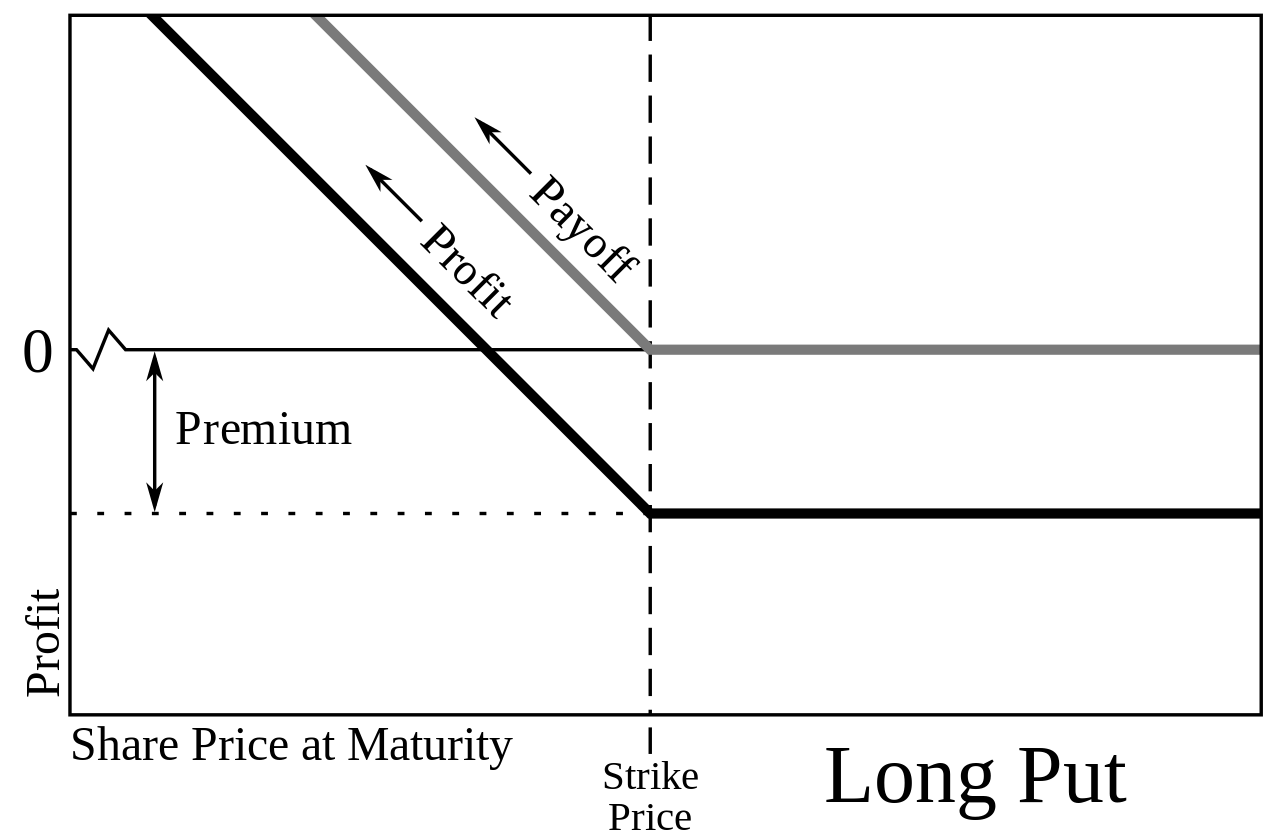
\includegraphics[scale=0.12]{Long_put_option}
\end{align*}

\vspace{0.15cm}

The profit from buying (going "long" or "Long Put") a put option is shown in the figure above

\begin{align*}
\centering
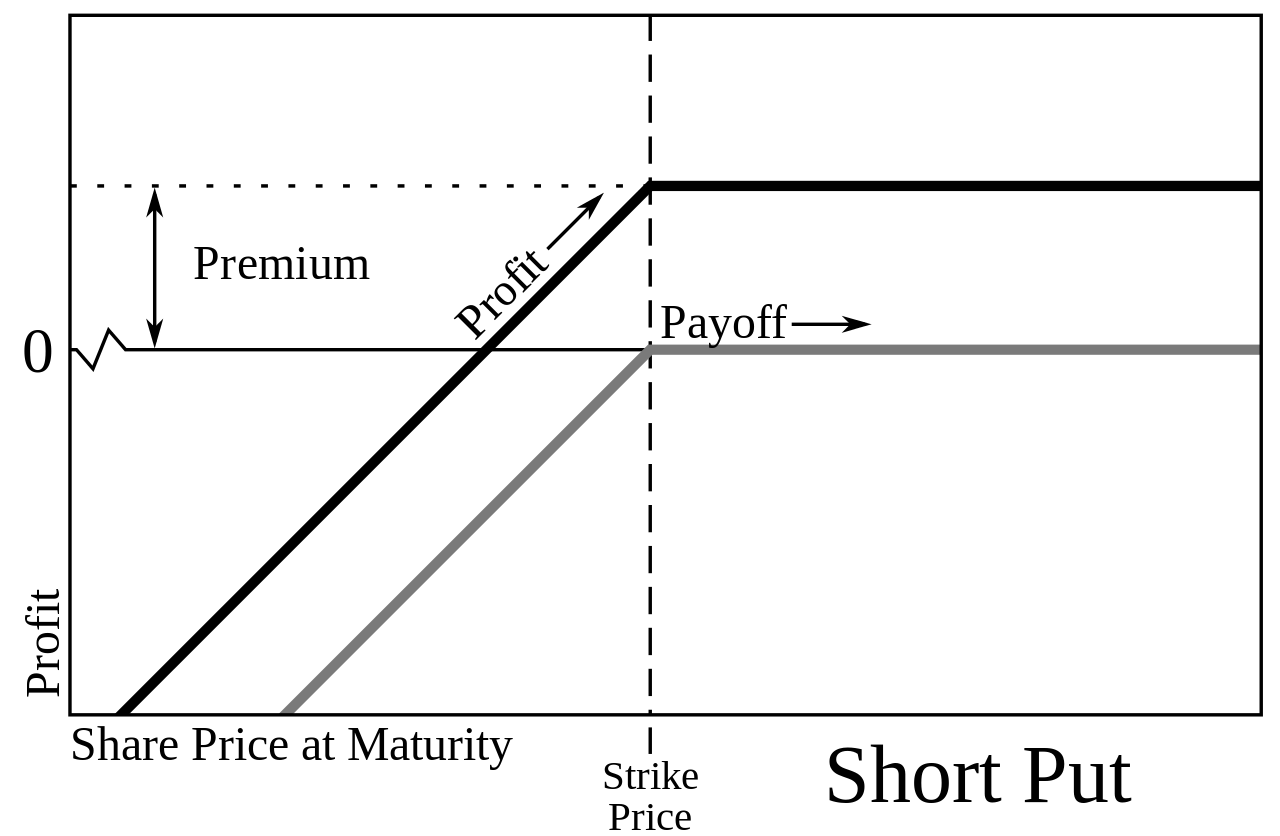
\includegraphics[scale=0.12]{Short_put_option}
\end{align*}

\vspace{0.15cm}

The profit from selling (going short or writing) a put option is shown in the figure above

\vspace{0.15cm}

A \textbf{European} option may be exercised only at the expiration date of the option, i.e. at a single pre-defined point in time

\vspace{0.15cm}

An \textbf{American} option on the other hand may be exercised at any time before the expiration date. This means that you could be put in an akward position of having to fulfill your obligations before you expect in some cases.

\vspace{0.15cm}

the payoff is

\vspace{0.15cm}

$\max\{(S-K), 0\}$, for a call option

$\max\{(K-S), 0\}$, for a put option

\vspace{0.15cm}

where $K$ is the strike price, and $S$ is the spot price

\vspace{0.15cm}
In options trading, a \textbf{vertical spread} is an options strategy involving buying and selling of multiple options of the same underlying security, same expiration date, but at different strike prices.
\vspace{0.15cm}

A \textbf{bull call spread} is constructed by buying a call option with a lower strike price (K), and selling another call option with a higher strike price.

\vspace{0.15cm}

Often the call with the lower exercise price will be at-the-money while the call with the higher exercise price is out-of-the-money. Both calls must have the same underlying security and expiration month. If the bull call spread is done so that both the sold and bought calls expire on the same day, it is a vertical debit call spread.

\vspace{0.15cm}
 
Break even point= Lower strike price + Net premium paid

\vspace{0.15cm}

notice that in the bull-call-spread you will be definitely paying a net  premium.
You can also construct a bull - put - spread with puts - in this case you will recieve a net premium ( i haven't analyzed this but it should be straightforward)


\begin{align*}
\centering
\includegraphics[scale=0.4]{bull_call_spread2}
\end{align*}

\vspace{0.15cm}

A \textbf{bear call spread} is entered by buying call options of a certain strike price and selling the same number of call options of lower strike price (in the money) on the same underlying security with the same expiration month. 

\vspace{0.15cm}

Example:

Consider a stock that costs \$100 per share, with a call option with a strike price of \$105 for \$2 and a call option with a strike price of \$95 for \$7. To implement a bear call spread, one 

\vspace{0.15cm}

buys the \$105 call option, paying a premium of \$2, and

\vspace{0.15cm}

sells the \$95 call option, making a premium of \$7.

The total profit after this initial options trading phase will be \$5. 
After the options reach expiration, the options may be exercised. If the stock price ends at a price (P) below or equal to \$95, neither option will be exercised and your total profit will be the \$5 per share from the initial options trade. 
If the stock price ends at a price (P) above or equal to \$105, both options will be exercised and your total profit per is equal to the sum of \$5 from the original options trading, a loss of (P - \$95) from the sold option, and a gain of (P - \$105) from the bought option. Total profits will be (\$5 - (P - \$95) + (P - \$105)) = -\$5 per share (i.e. a loss of \$5 per share). The loss is due to speculation that the price would go down but it actually did not. 

\begin{align*}
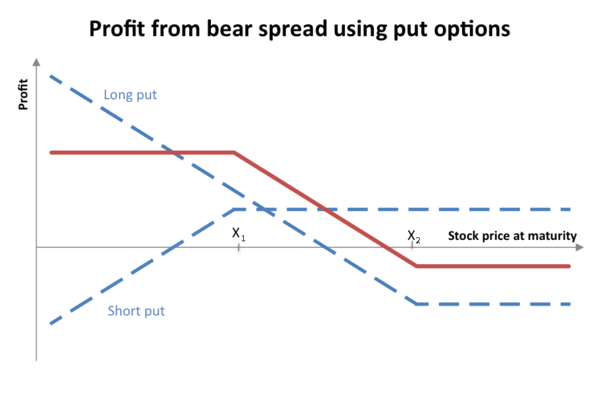
\includegraphics[scale=0.6]{bear_call_spread}
\end{align*}

\vspace{0.15cm}

A ``\textbf{conversion}'' position is:

\vspace{0.15cm}

\begin{itemize}
	\item short  a call option,
	\item long  a put option, and 
	\item long the underlying
\end{itemize}

\vspace{0.15cm}

The call and put have the same strike  value and expiration date. The resulting portfolio is delta neutral.

\vspace{0.15cm}

One reason a trader may take this position would be to extend the holding period of the underlying position for capital gains tax purposes, while locking in the current price.

\vspace{0.15cm}

A ``\textbf{reversal}'' position is:

\vspace{0.15cm}

\begin{itemize}
	\item long  a call option,
	\item short  a put option, and 
	\item short the underlying
\end{itemize}

\vspace{0.15cm}

\section{the greeks}

\vspace{0.15cm}

\textbf{$\alpha$ is Alpha} is a measure of the active return on an investment.
 active return refers to that segment of the returns in an investment portfolio that is due to active management decisions made by the portfolio manager. It does not include any return that is merely a function of the market's movement. The active return is calculated as the return of the portfolio minus some benchmark return, e.g. from an index fund such as the S\&P 500. If $R_p$ denotes the return for the portfolio and $R_b$ denotes the return for the benchmark, then the active return is given by $R_{p}-R_{b}$ , and can be either positive or negative
 
 \vspace{0.15cm}

\textbf{beta}, $\beta$, is a measure of the risk arising from exposure to general market movements as opposed to idiosyncratic factors. The market portfolio of all investable assets has a beta of exactly 1. A beta below 1 can indicate either an investment with lower volatility than the market, or a volatile investment whose price movements are not highly correlated with the market. An example of the first is a treasury bill: the price does not go up or down a lot, so it has a low beta. An example of the second is gold. The price of gold does go up and down a lot, but not in the same direction or at the same time as the market. A beta greater than 1 generally means that the asset both is volatile and tends to move up and down with the market. An example is a stock in a big technology company.

 \vspace{0.15cm}
 
 $$r_a = \alpha + \beta r_b$$
 
  \vspace{0.15cm}

$r_a$ is the return of the asset

 \vspace{0.15cm}
 
 $\alpha$ is the active return
 
  \vspace{0.15cm}
 
 $r_b$ is the return of the benchmark

\vspace{0.15cm}

This can be written as


$$\beta = \rho_{a,b} \frac{\sigma_a}{\sigma_b}$$

where $\rho_{a,b}$ is the correlation between the returns 

 \vspace{0.15cm}
 
\textbf{$\sigma$ is volatility:}  degree of variation of a trading price series over time as measured by the standard deviation of logarithmic returns. We often look at it from the perspective of a random walk in terms of the time-dependence, which is square root T. Implied volatility is the volatility derived from the price of an option of the underlying. E.g. the option price may suggest a future volatility for some time period related to the expiration date.

\vspace{0.15cm}

``annualized" volatility $\sigma_{annually}$ is the standard deviation of an instrument's yearly log returns. Notice, this shouldn't depend too much on the sampling rate of the data. e.g. you need maybe a few measurements per day or something, assuming, that you don't miss alot of crazy intra-day swings.

\vspace{0.15cm}

The generalized volatility $\sigma_{T}$ for time horizon T in years is expressed as:

\vspace{0.15cm}

$$\sigma_\text{T} = \sigma_\text{annually} \sqrt{T}$$

\vspace{0.15cm}

Therefore, if the daily logarithmic returns of a stock have a standard deviation of $\sigma_{daily}$ and the time period of returns is P in trading days, the annualized volatility is

\vspace{0.15cm}

$$\sigma_\text{P} = \sigma_\text{daily} \sqrt{P}$$

\vspace{0.15cm}

A common assumption is that P = 252 trading days in any given year. Then, if $\sigma_\text{daily} = 0.01$, the annualized volatility is

\vspace{0.15cm}

$$\sigma_\text{annually} = 0.01 \sqrt{252} = 0.1587$$

\vspace{0.15cm}

The monthly volatility (i.e., T = 1/12 of a year or P = 252/12 = 21 trading days) would be

\vspace{0.15cm}

$$\sigma_\text{monthly} = 0.1587 \sqrt{\tfrac{1}{12}} = 0.0458$$

\vspace{0.15cm}

$$\sigma_\text{monthly} = 0.01 \sqrt{\tfrac{252}{12}} = 0.0458$$

\vspace{0.15cm}

\begin{itemize}
	\item \textbf{actual current volatility} of a financial instrument for a specified period (for example 30 days or 90 days), based on historical prices over the specified period with the last observation the most recent price
	\item \textbf{actual historical volatility} which refers to the volatility of a financial instrument over a specified period but with the last observation on a date in the past 
	\item \textbf{historical implied volatility} which refers to the implied volatility observed from historical prices of the financial instrument (normally options)
	\item current implied volatility which refers to the implied volatility observed from current prices of the financial instrument
	\item future implied volatility which refers to the implied volatility observed from future prices of the financial instrument
\end{itemize}


\vspace{0.15cm}

\textbf{theta}, $\Theta=\tfrac {\partial V}{\partial t}$,  measures the sensitivity of the value of the derivative to the passage of time (see Option time value): the ``time decay" 

$$\textrm{Time Value} = \textrm{Option Value} - \textrm{Intrinsic Value}$$

\vspace{0.15cm}

\textbf{delta}, $\Delta$, measures the rate of change of the theoretical option value with respect to changes in the underlying asset's price, $\tfrac {\partial V}{\partial S}$ For a vanilla option, delta will be a number between 0.0 and 1.0 for a long call (or a short put) and 0.0 and −1.0 for a long put (or a short call); depending on price, a call option behaves as if one owns 1 share of the underlying stock (if deep in the money), or owns nothing (if far out of the money), or something in between, and conversely for a put option. The difference between the delta of a call and the delta of a put at the same strike is close to but not in general equal to one, but instead is equal to the inverse of the discount factor.

\vspace{0.15cm}

if a stock option has a delta value of 0.65, this means that if the underlying stock increases in price by \$1 per share, the option on it will rise by \$0.65 per share, all else being equal

\vspace{0.15cm}

These numbers are commonly presented as a percentage of the total number of shares represented by the option contract(s). This is convenient because the option will (instantaneously) behave like the number of shares indicated by the delta. For example, if a portfolio of 100 American call options on XYZ each have a delta of 0.25 (=25\%), it will gain or lose value just like 2,500 shares of XYZ as the price changes for small price movements (100 option contracts covers 10,000 shares). The sign and percentage are often dropped – the sign is implicit in the option type (negative for put, positive for call) and the percentage is understood. The most commonly quoted are 25 delta put, 50 delta put/50 delta call, and 25 delta call. 50 Delta put and 50 Delta call are not quite identical, due to spot and forward differing by the discount factor, but they are often conflated. 

\vspace{0.15cm}

Delta is always positive for long calls and negative for long puts (unless they are zero). The total delta of a complex portfolio of positions on the same underlying asset can be calculated by simply taking the sum of the deltas for each individual position – delta of a portfolio is linear in the constituents. Since the delta of underlying asset is always 1.0, the trader could delta-hedge his entire position in the underlying by buying or shorting the number of shares indicated by the total delta. For example, if the delta of a portfolio of options in XYZ (expressed as shares of the underlying) is +2.75, the trader would be able to delta-hedge the portfolio by selling short 2.75 shares of the underlying. This portfolio will then retain its total value regardless of which direction the price of XYZ moves. (Albeit for only small movements of the underlying, a short amount of time and not-withstanding changes in other market conditions such as volatility and the rate of return for a risk-free investment). 

\vspace{0.15cm}

The (absolute value of) Delta is close to, but not identical with, the percent moneyness of an option, i.e., the implied probability that the option will expire in-the-money (if the market moves under Brownian motion in the risk-neutral measure).[5] For this reason some option traders use the absolute value of delta as an approximation for percent moneyness. For example, if an out-of-the-money call option has a delta of 0.15, the trader might estimate that the option has approximately a 15\% chance of expiring in-the-money. Similarly, if a put contract has a delta of −0.25, the trader might expect the option to have a 25\% probability of expiring in-the-money. At-the-money calls and puts have a delta of approximately 0.5 and −0.5 respectively with a slight bias towards higher deltas for ATM calls. The actual probability of an option finishing in the money is its dual delta, which is the first derivative of option price with respect to strike.

\vspace{0.15cm}

Given a European call and put option for the same underlying, strike price and time to maturity, and with no dividend yield, the sum of the absolute values of the delta of each option will be 1 – more precisely, the delta of the call (positive) minus the delta of the put (negative) equals 1. This is due to put–call parity: a long call plus a short put (a call minus a put) replicates a forward, which has delta equal to 1. 
If the value of delta for an option is known, one can calculate the value of the delta of the option of the same strike price, underlying and maturity but opposite right by subtracting 1 from a known call delta or adding 1 to a known put delta. $\Delta (call)-\Delta (put)=1$
For example, if the delta of a call is 0.42 then one can compute the delta of the corresponding put at the same strike price by 0.42 − 1 = −0.58. To derive the delta of a call from a put, one can similarly take −0.58 and add 1 to get 0.42. 

\vspace{0.15cm}

\textbf{rho}, $\rho=\tfrac {\partial V}{\partial r}$, measures the sensitivity by the value of the derivative to the interest rate.

 \vspace{0.15cm}
 
\textbf{Vega} $=\tfrac {\partial V}{\partial \sigma}$ measures the sensitivity of the value of the derivative to the underlying's volatility. Vega is typically expressed as the amount of money per underlying share that the option's value will gain or lose as volatility rises or falls by 1\%. All options (both calls and puts) will gain value with rising volatility



\section{Net present value}

It's important to understand that money has a \textit{time value}. When considering cash flows, you need to consider when you get paid. A promise of 1000 in 10 years is worth less than 1000 handed to you right now. This is very important!

Each cash inflow/outflow is discounted back to its present value (PV). Then all are summed. Therefore, NPV is the sum of all terms,

\vspace{0.15cm}

$\frac{R_t}{(1+i)  ^{t}}$

\vspace{0.15cm}

where

\vspace{0.15cm}

$t$ – the time of the cash flow

\vspace{0.15cm}

$i$ – the discount rate (not in the sense below) or opportunity cost, i.e. the rate of return that could be earned per unit of time on an opportunity cost investment with similar risk

\vspace{0.15cm}

$R_t$ – the net cash flow i.e. cash inflow cash outflow, at time $t$. For educational purposes, $R_0$is commonly placed to the left of the sum to emphasize its role as (minus) the investment.

\vspace{0.15cm}

this is quite useful for planning long term projects. simple example, is the powerball lottery payment of 285 million is the NPV of a total of 20 25 million payments paid out over 20 years - the sum is 500 million but money later is worth less than money now!

\vspace{0.15cm}

\section{Various types of interest rates}

\vspace{0.25cm}

first of all, one \textbf{basis point} is a \textit{difference of} $1\textrm{bp}= 0.0001$ or $0.01\%$. Like percentage points, basis points avoid the ambiguity between relative and absolute discussions about interest rates by dealing only with the absolute change in numeric value of a rate. For example, if a report says there has been a "1\% increase" from a 10\% interest rate, this could refer to an increase either from 10\% to 10.1\% (relative, 1\% of 10\%), or from 10\% to 11\% (absolute, 1\% plus 10\%). However, if the report says there has been a "100 basis point increase" from a 10\% interest rate, then the interest rate of 10\% has increased by 1.00\% (the absolute change) to an 11\% rate.

\vspace{0.15cm}

\textbf{risk free rate}: The return on domestically held short-dated government bonds is normally perceived as a good proxy for the risk-free rate. In business valuation the long-term yield on the US Treasury coupon bonds is generally accepted as the risk-free rate of return. However, governments can default and there can be inflation, so really there is no true "risk free" rate absolutely.

\vspace{0.15cm}

\textbf{discount rate}: (aka the base rate, the repo rate) is the rate at which central bank lends to institutions (banks) usually  higher than the federal funds target rate.

\vspace{0.15cm}

\textbf{federal funds rate}: the rate at which US institutions lend reserve balances to each other \textit{overnight} on an \textit{uncollateralized} basis. Reserve balances are held at the federal reserve to meet federal reserve requirements. This rate has a target set by the fed.

\vspace{0.15cm}

\textbf{libor rate}: The London Inter-bank Offered Rate is an interest-rate average calculated from estimates submitted by the leading banks in London of what rates they would charge other banks. Libor rates are calculated for five currencies and seven borrowing periods ranging from overnight to one year and are published each business day by Thomson Reuters.[6] Many financial institutions, mortgage lenders and credit card agencies set their own rates relative to it. At least 350 trillion in derivatives and other financial products are tied to Libor. Libor is going away in 2021 and something else will take its place. Sometimes it can be considered as the risk-free-rate.

\vspace{0.15cm}

\textbf{prime rate}: the rate at which banks lend to their favorite customers.

\vspace{0.15cm}


\section{Black Scholes}

\vspace{0.15cm}

Assumptions on the assets

\vspace{0.15cm}

\begin{itemize}
	\item  The rate of return on the riskless asset is constant (risk-free rate)
	\item  The instantaneous log return of stock price is an infinitesimal random walk with drift; more precisely, it is a geometric Brownian motion, and we will assume its drift and volatility are constant (if they are time-varying, we can deduce a suitably modified Black–Scholes formula quite simply, as long as the volatility is not random).
	\item The stock does not pay a dividend
\end{itemize}

\vspace{0.15cm}

Assumptions on the market

\vspace{0.15cm}

\begin{itemize}
	\item There is no arbitrage opportunity (i.e., there is no way to make a riskless profit)
	\item It is possible to borrow and lend any amount, even fractional, of cash at the riskless rate.
	\item It is possible to buy and sell any amount, even fractional, of the stock (this includes short selling).
	\item The above transactions do not incur any fees or costs (i.e., frictionless market)
\end{itemize}

\vspace{0.15cm}

ok, so first thing is LOL, at some of these assumptions which are obviously not true. We will consider the effects later. 

\vspace{0.15cm}

 For the special case of a European call or put option, Black and Scholes showed that "it is possible to create a hedged position, consisting of a long position in the stock and a short position in the option, whose value will not depend on the price of the stock"
 
 \vspace{0.15cm}

The notation used throughout this page will be defined as follows:

\vspace{0.15cm}

$S(t)$, the spot price of the underlying asset at time ``t''.;
 
\vspace{0.15cm}

$V(S, t)$, the price of the option as a function of the underlying asset ``S'', at time ``t'';
 
\vspace{0.15cm}

$C(S, t)$, the price of a European call option and $P(S, t)$ the price of a European put option;
 
\vspace{0.15cm}

$K$, the strike price of the option, also known as the exercise price;
 
\vspace{0.15cm}

$r$, the annualized risk-free interest rate, continuously compounded, also known as the force of interest;
 
\vspace{0.15cm}

$\mu$, the drift rate of $S$, annualized;
 
\vspace{0.15cm}

$\sigma$, the standard deviation of the stock's returns; this is the square root of the quadratic variation of the stock's log price process;
 
\vspace{0.15cm}

$t$, a time in years; we generally use: now $= 0 $, expiry $ = T $;
 
\vspace{0.15cm}

$\Pi$, the value of the portfolio.
 
\vspace{0.15cm}

We will use $N(x)$ to denote the standard normal cumulative distribution function,
$N(x) = \frac{1}{\sqrt{2\pi}}\int_{-\infty}^x e^{-z^2/2}\, dz$
 
\vspace{0.15cm}

$N'(x)$ will denote the standard normal probability density function,
$N'(x) = \frac{1}{\sqrt{2\pi}} e^{-x^2/2}$
 
\vspace{0.15cm}

the Black–Scholes formula for the price of a vanilla call option (or put option) can be interpreted by decomposing a call option into an asset-or-nothing call option minus a cash-or-nothing call option. A cash-or-nothing would be basically a bet that the assett is above or below the strike price with no asset exchanged. An asset-or-nothing would be a bet that it is above or below the strike price with no premium paid for this, someone will either get the assett (at the strike price) or not. These are called ``binary options"

\vspace{0.15cm}

The value of a call option for a non-dividend-paying underlying stock in terms of the Black–Scholes parameters is:

\vspace{0.15cm}

\begin{align}
C(S_t, t)  = N(d_1)S_t - N(d_2) PV(K) \\
d_1  = \frac{1}{\sigma\sqrt{T - t}}\left[\ln\left(\frac{S_t}{K}\right) + \left(r + \frac{\sigma^2}{2}\right)(T - t)\right] \\
d_2  = d_1 - \sigma\sqrt{T - t} \\
PV(K)  =Ke^{-r(T - t)}
\end{align}

\vspace{0.15cm}


The price of a corresponding put option based on put–call parity is:

\vspace{0.15cm}

\begin{align}
P(S_t, t) = Ke^{-r(T - t)} - S_t + C(S_t, t) \\
= N(-d_2) Ke^{-r(T - t)} - N(-d_1) S_t
\end{align}


\section{swaps}

These are basically situations where each party swaps the interest cash flow on a principal. The principal is not exchanged, it's basically an agreement to swap to cash flows. One of the cash flows is often fixed, while the other depends on the currency or some floating interest rate.

\section{Sharpe ratio}

The return of an asset compared to the risk-free rate adjusted by volatility of the risky asset

\section{contango backwardation}

This is for futures contracts which you probably don't want to get into but contango/backwardation basically says the future price is higher/lower than the spot (current price)

\section{bucket shop}

"Bucket shop" is a defined term in the many U.S. states that criminalize the operation of a bucket shop. Typically the criminal law definition refers to an operation in which the customer is sold what is supposed to be a derivative interest in a security or commodity future, but there is no transaction made on any exchange. The transaction goes "in the bucket" and is never executed. Because no trading of actual securities occurs, the customer is essentially betting against the bucket shop operator in a game based on abstract security prices. While trading in a legitimate exchange also provides a similar game or wagering aspect, the one distinctive characteristic of a bucket shop is the mimicry of trading securities when no actual securities are traded. The bucket shop's exchange is a fiction, which the parties agree to imagine as following the events occurring in a real exchange. Alternatively, the bucket shop operator literally 'plays the bank,' as in a gambling house, against the customer


\end{multicols}
\end{document}